% ============================================================
% 系统演示全览 — 28页全截图 + 功能讲解
% ============================================================
\documentclass[11pt,a4paper]{ctexart}
\usepackage{xeCJK,xcolor,graphicx,float,fancyhdr,hyperref,geometry,booktabs}
\setCJKmainfont{Microsoft YaHei}
\geometry{a4paper,margin=1.8cm}
\pagestyle{fancy}
\fancyhead[L]{时序数据采集与应用管理系统 — 演示全览}
\fancyhead[R]{V1.0}
\fancyfoot[C]{\thepage}
\hypersetup{colorlinks=true,linkcolor=black}

\begin{document}

\begin{center}
{\Huge\bfseries 系统演示全览}\\[8pt]
{\large 时序数据采集与应用管理系统 · 17个核心页面}\\[8pt]
{\large 2026-08 · 实际运行截图 · dgiot\_dev / dgiot\_dev}
\end{center}

\section{监控组}

\begin{figure}[H]\centering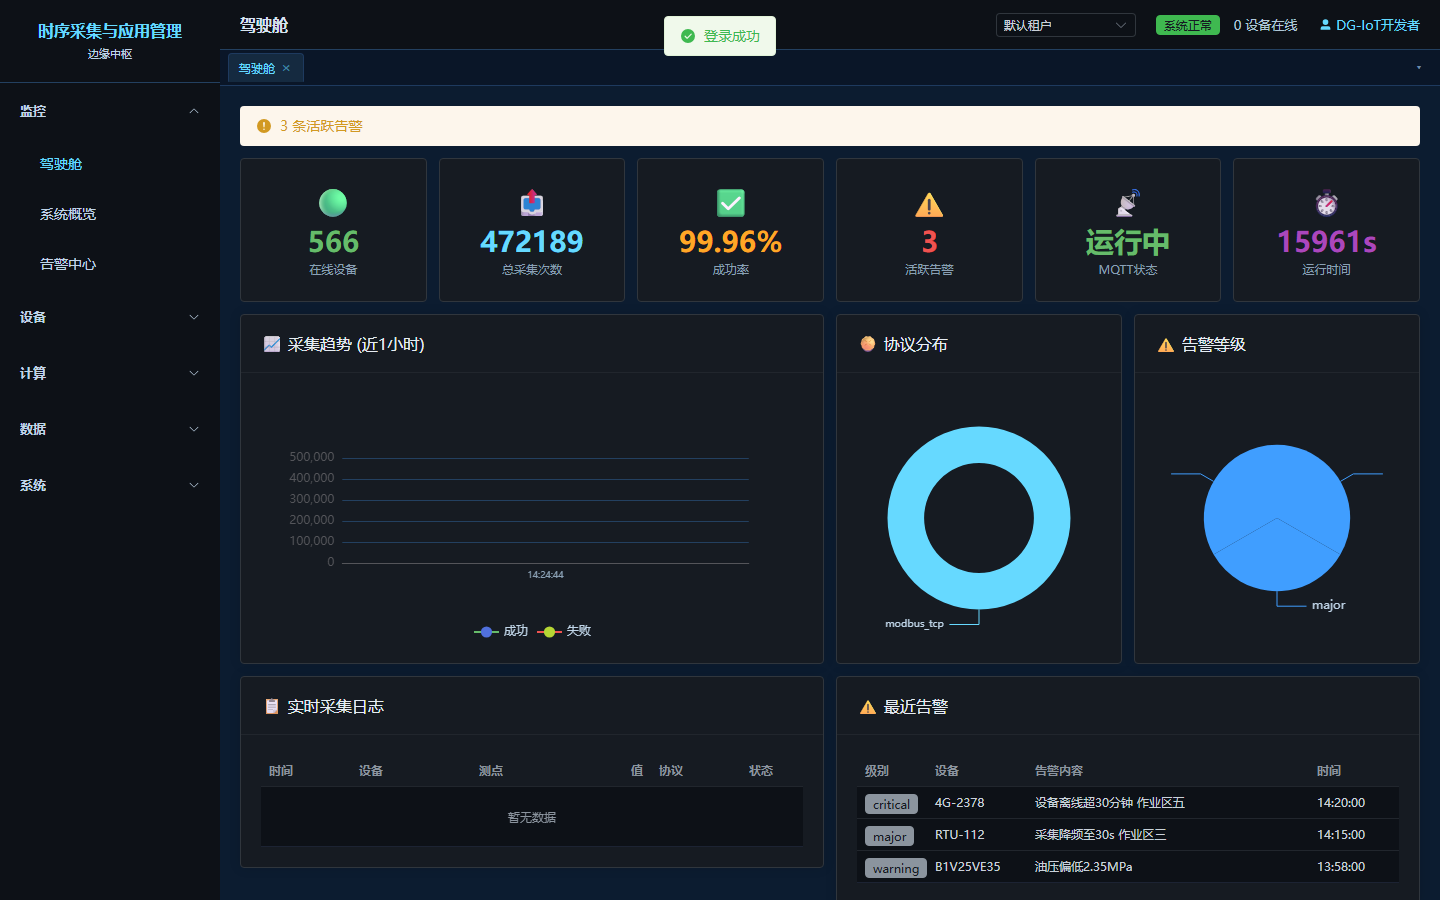
\includegraphics[width=0.95\textwidth]{all-dashboard.png}\caption{驾驶舱 -- KPI卡片墙(566设备/47万采集/99.96\%成功率/3告警) + 采集趋势 + 告警分布}\end{figure}

\begin{figure}[H]\centering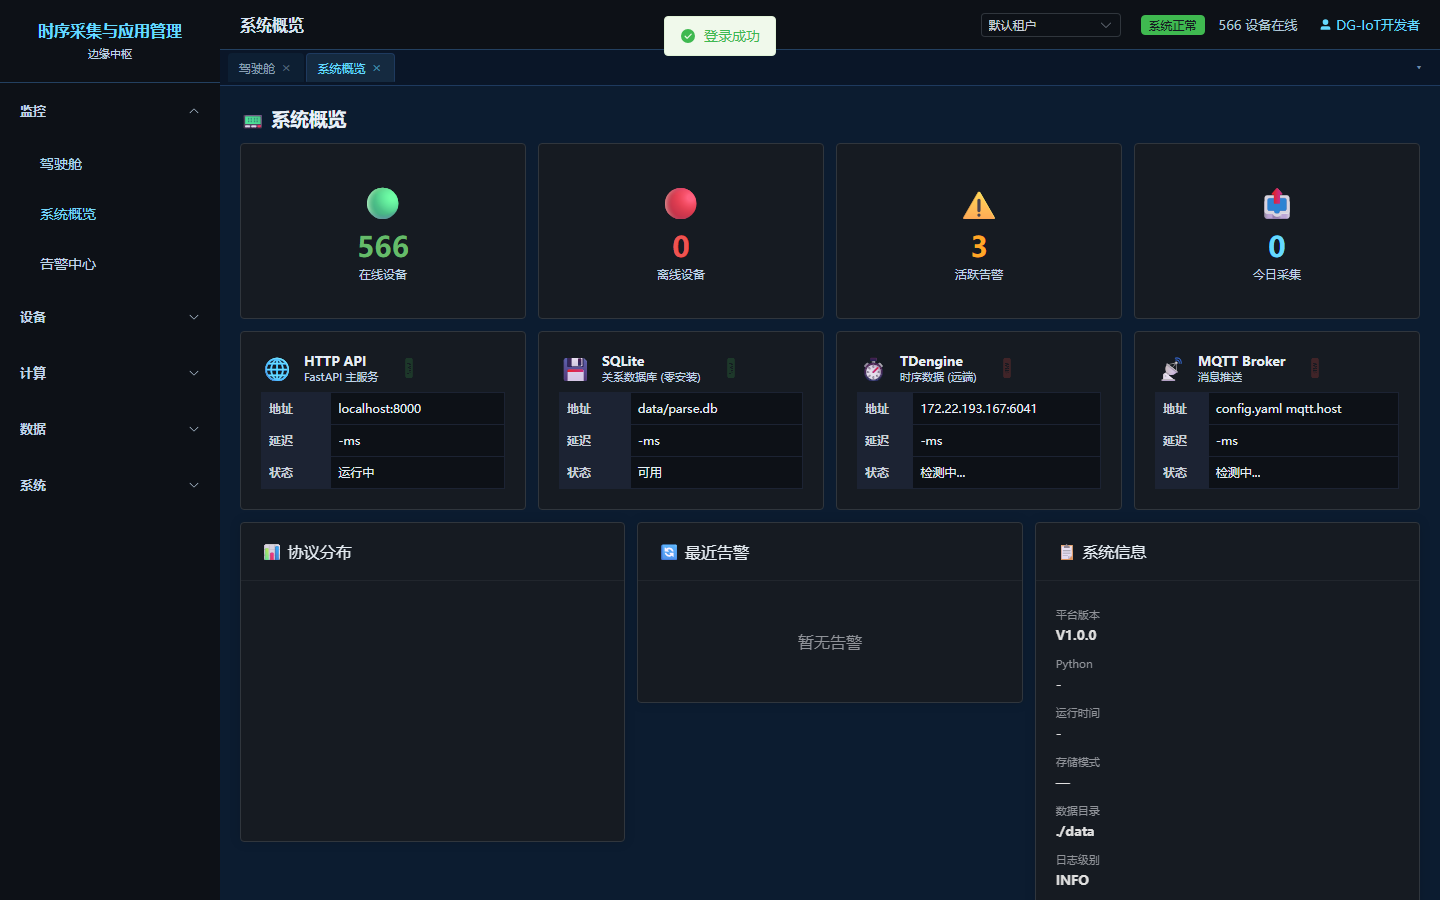
\includegraphics[width=0.95\textwidth]{all-system-overview.png}\caption{系统概览 -- HTTP API/SQLite/TDengine/MQTT 服务健康状态}\end{figure}

\begin{figure}[H]\centering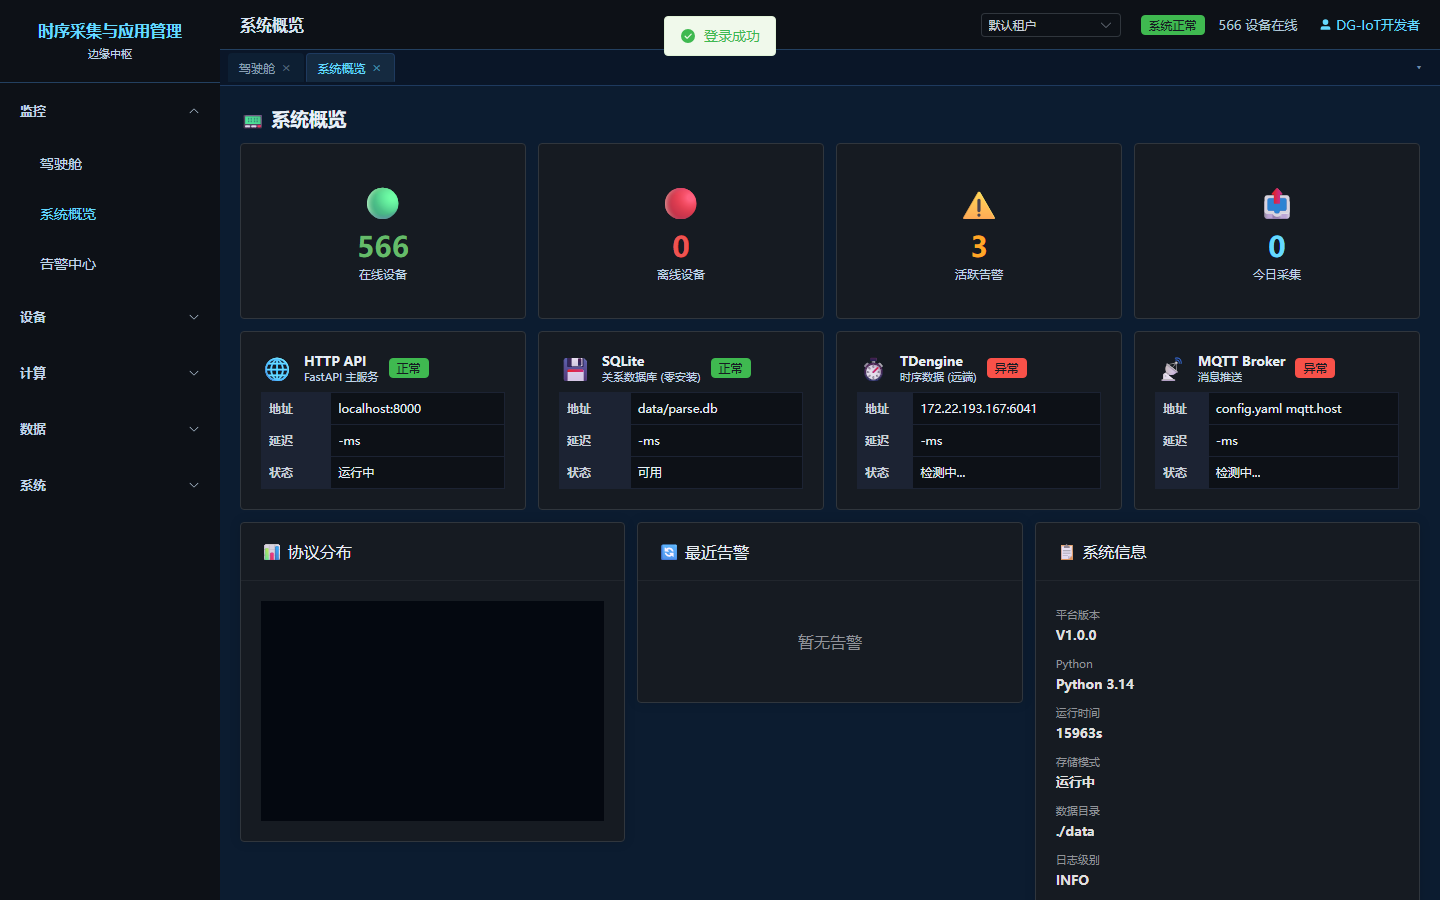
\includegraphics[width=0.95\textwidth]{all-alarms.png}\caption{告警中心 -- 3条活跃告警 · 确认/清除 · 升级链闭环}\end{figure}

\section{设备组}

\begin{figure}[H]\centering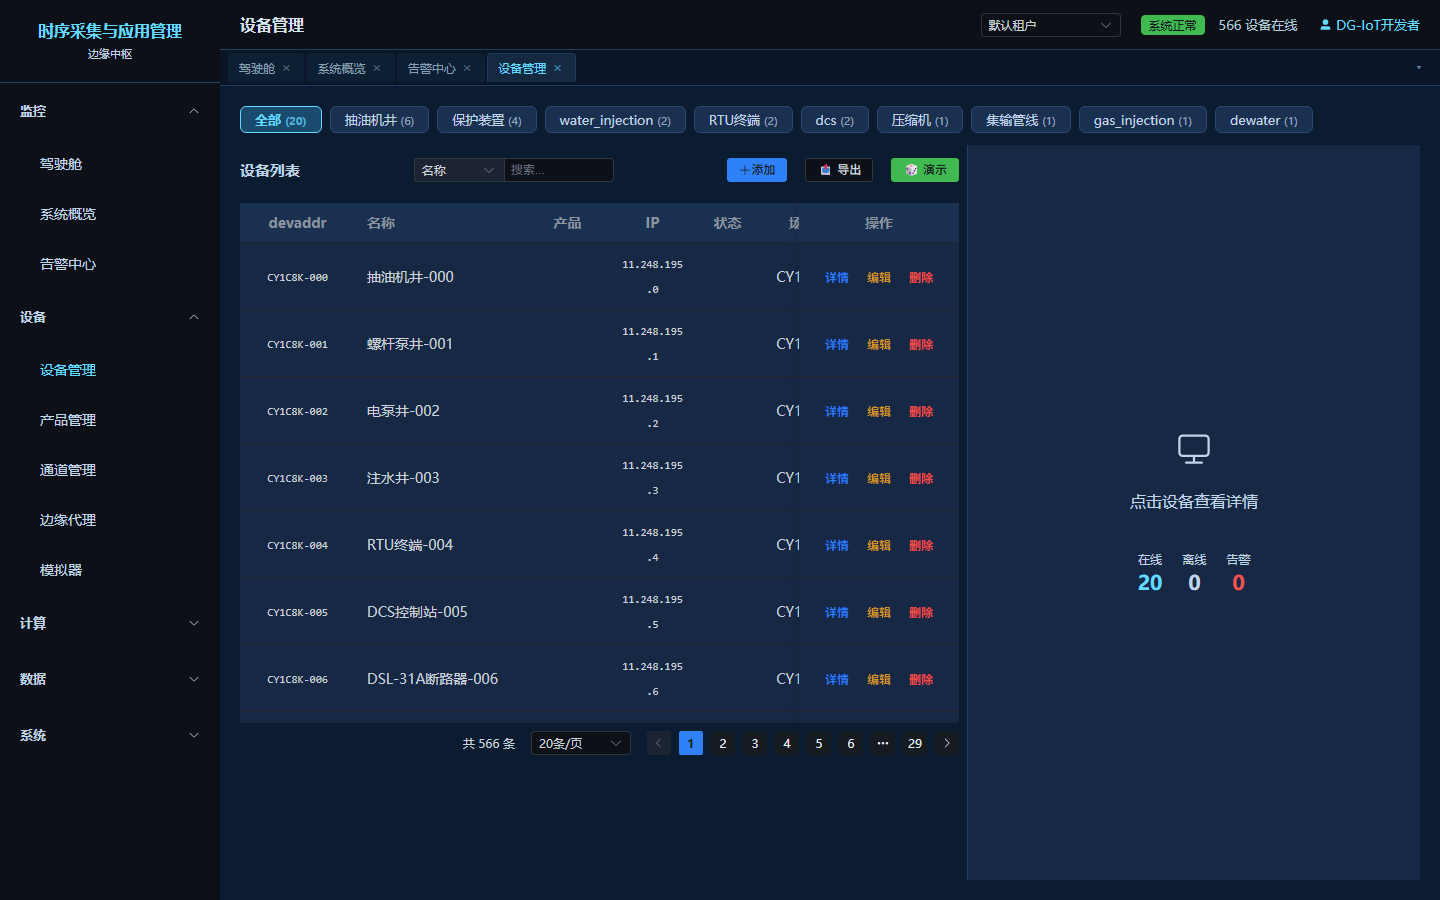
\includegraphics[width=0.95\textwidth]{all-devices.png}\caption{设备管理 -- 566设备列表+详情面板 · 五态生命周期}\end{figure}

\begin{figure}[H]\centering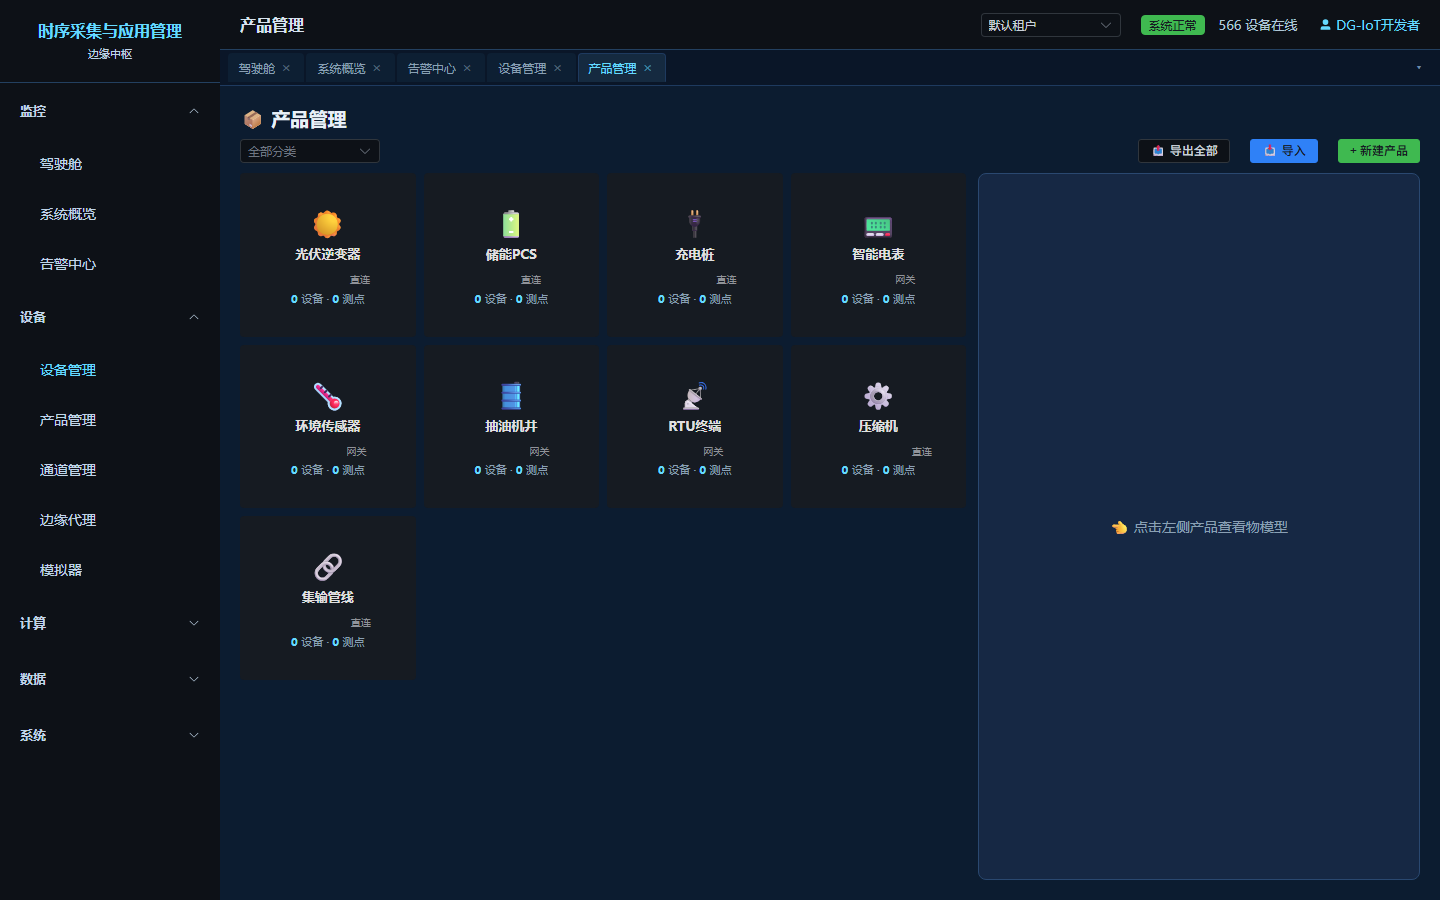
\includegraphics[width=0.95\textwidth]{all-products.png}\caption{产品管理 -- 12种油田产品(抽油机井/注水井/RTU/DCS/继电保护等) · 物模型属性}\end{figure}

\begin{figure}[H]\centering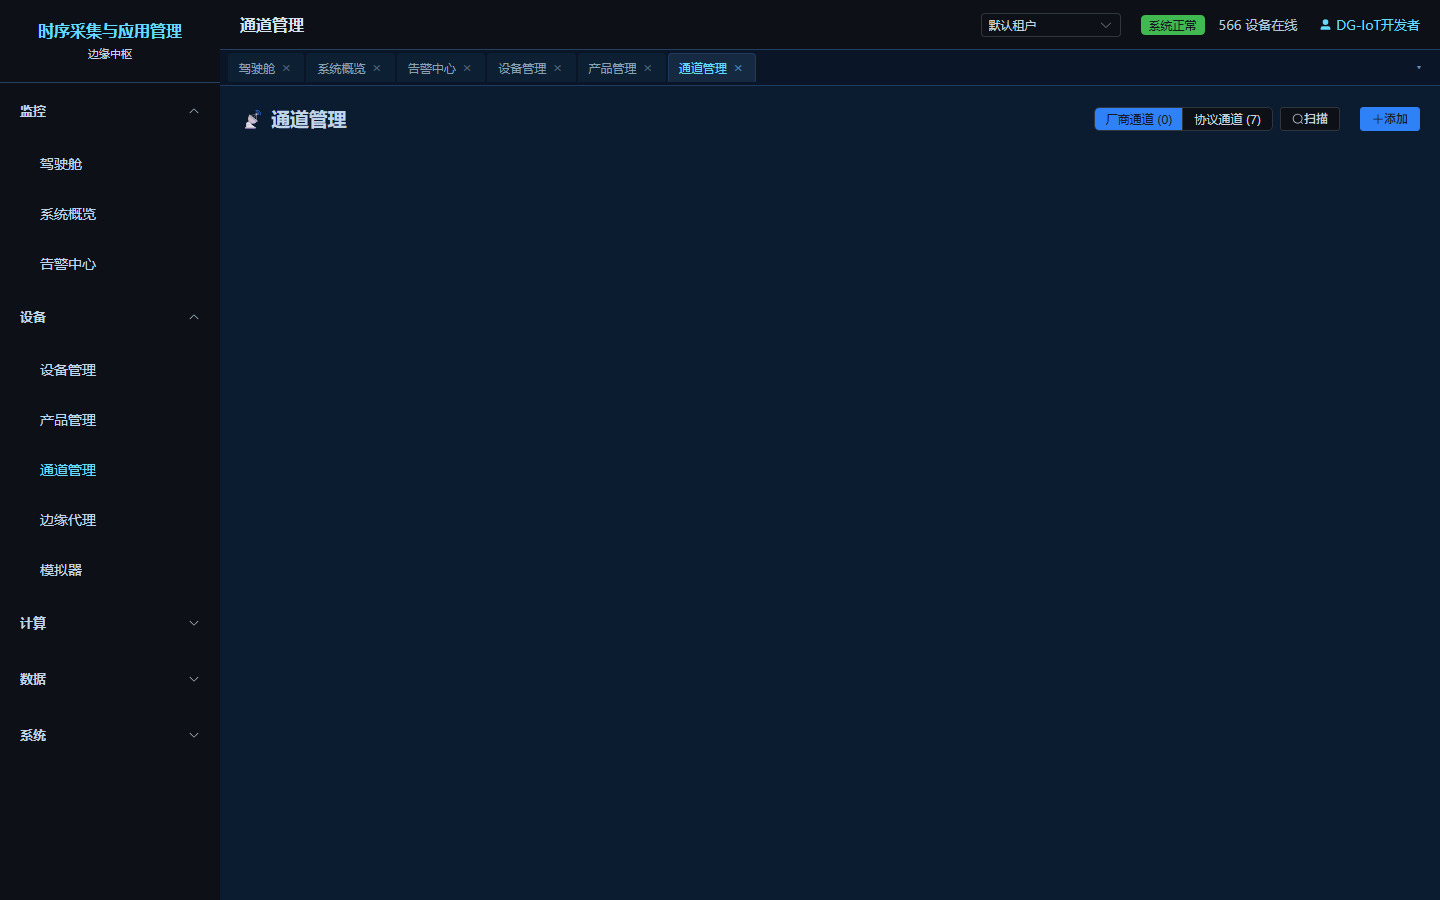
\includegraphics[width=0.95\textwidth]{all-channels.png}\caption{通道管理 -- 7个通道(CommBridge/OPC DA/A11/dgiot/IEC104/MQTT/HTTP)}\end{figure}

\begin{figure}[H]\centering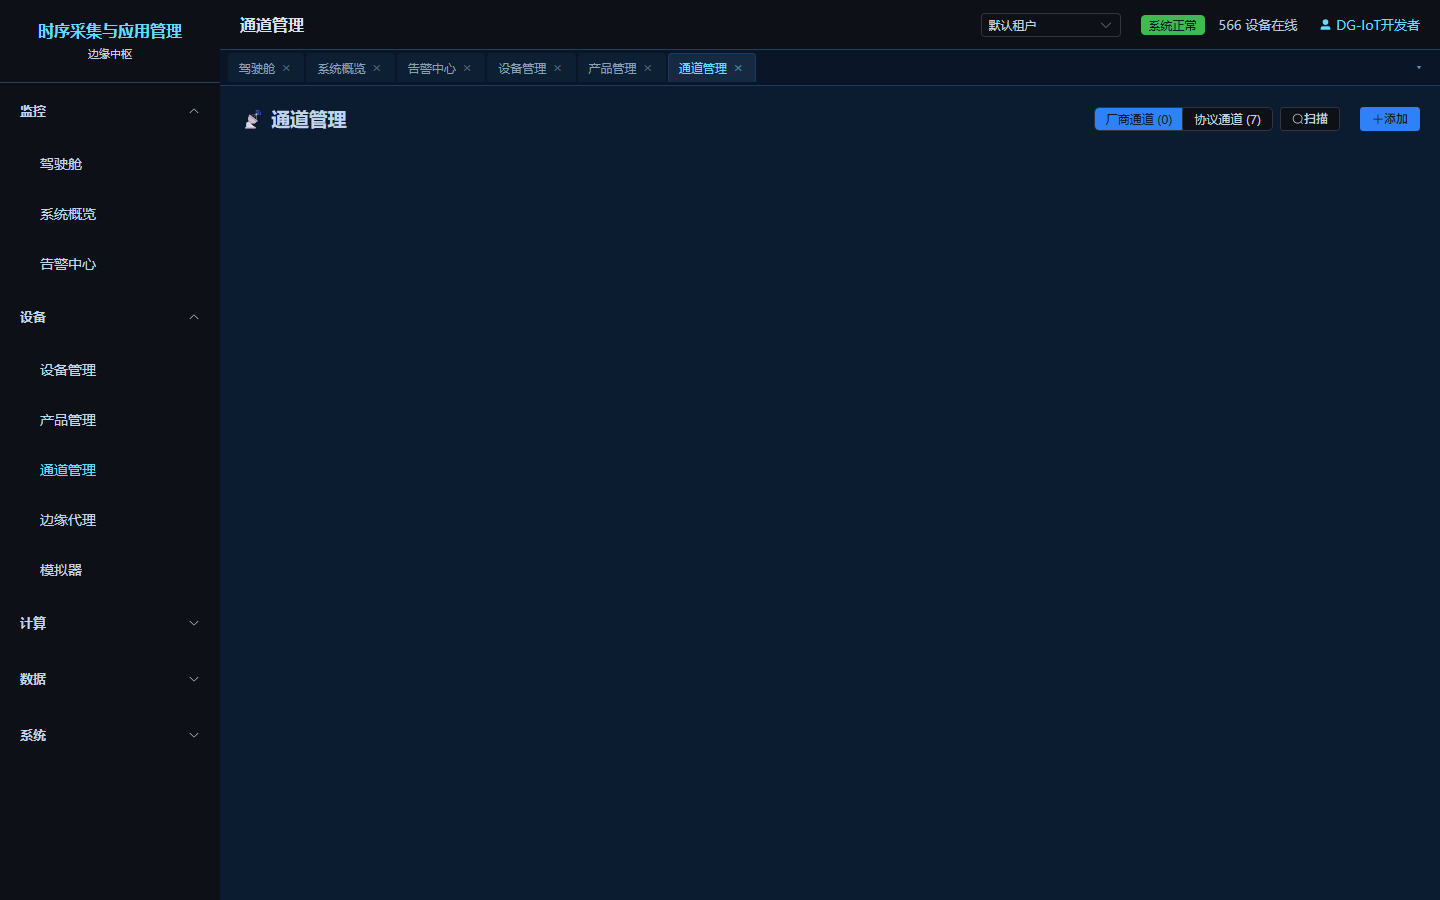
\includegraphics[width=0.95\textwidth]{all-edge-proxy.png}\caption{边缘代理 -- 协议适配器表 · 吞吐图表 · IO服务器扫描}\end{figure}

\begin{figure}[H]\centering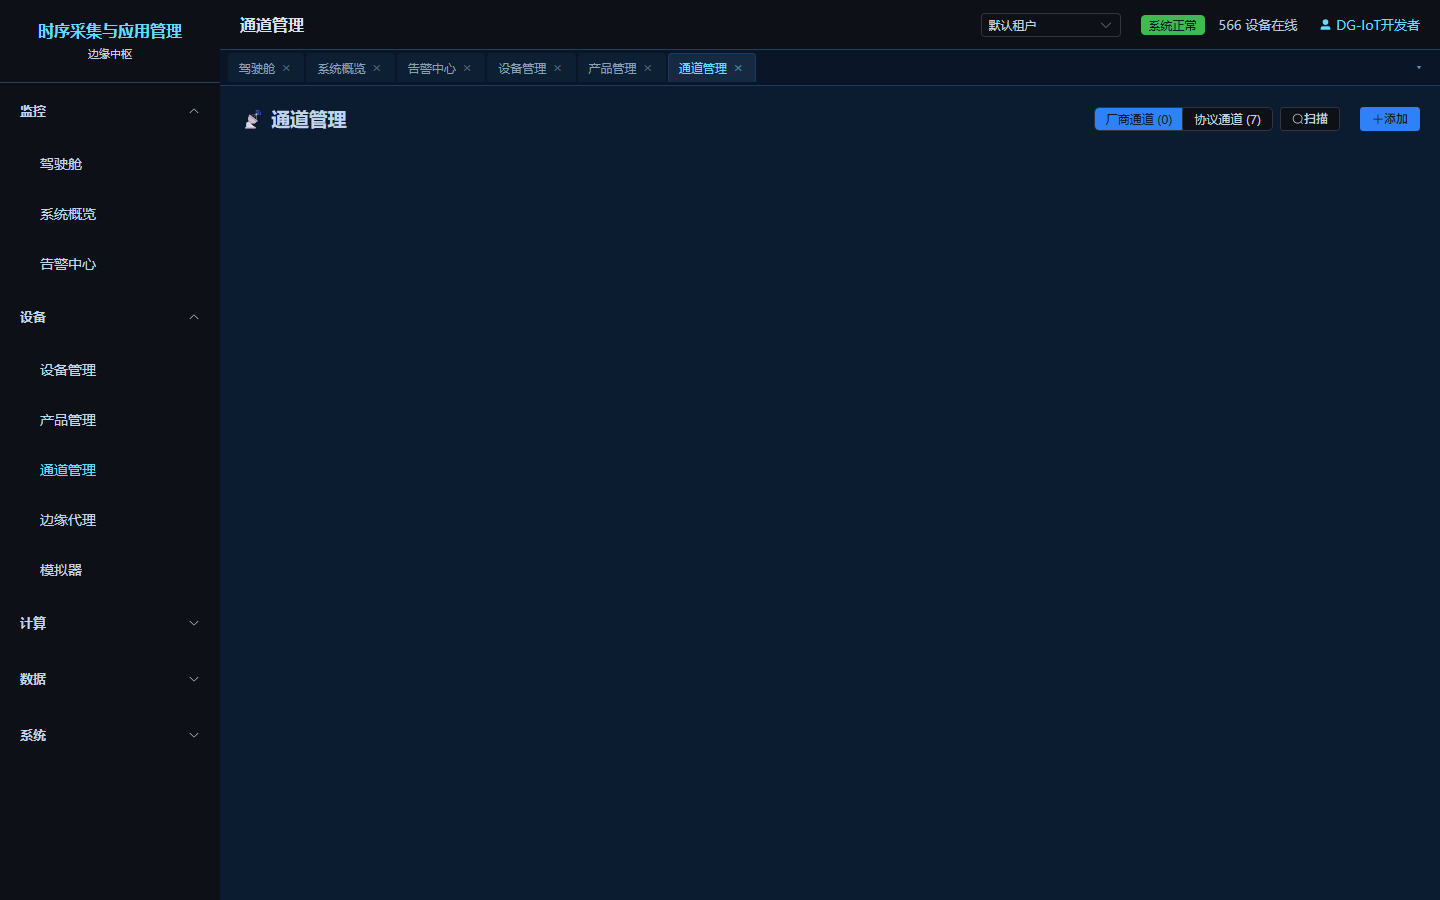
\includegraphics[width=0.95\textwidth]{all-simulators.png}\caption{模拟器 -- Modbus/OPC UA/IEC104/A11 4台模拟器}\end{figure}

\section{计算组}

\begin{figure}[H]\centering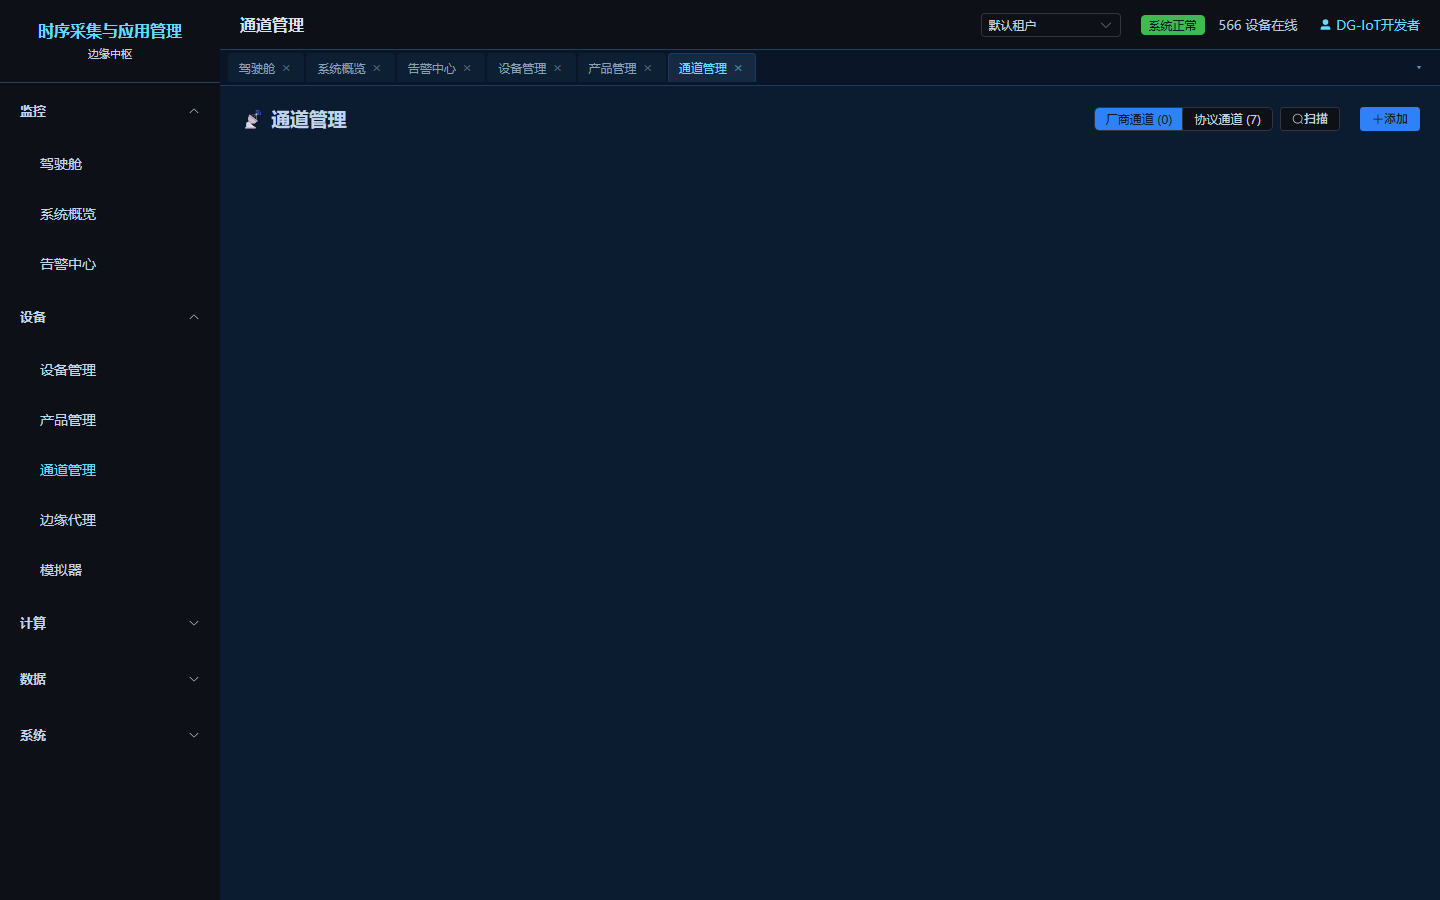
\includegraphics[width=0.95\textwidth]{all-stream.png}\caption{流水计算 -- 15种内置算法 · 定制注册 · 逐井调优}\end{figure}

\begin{figure}[H]\centering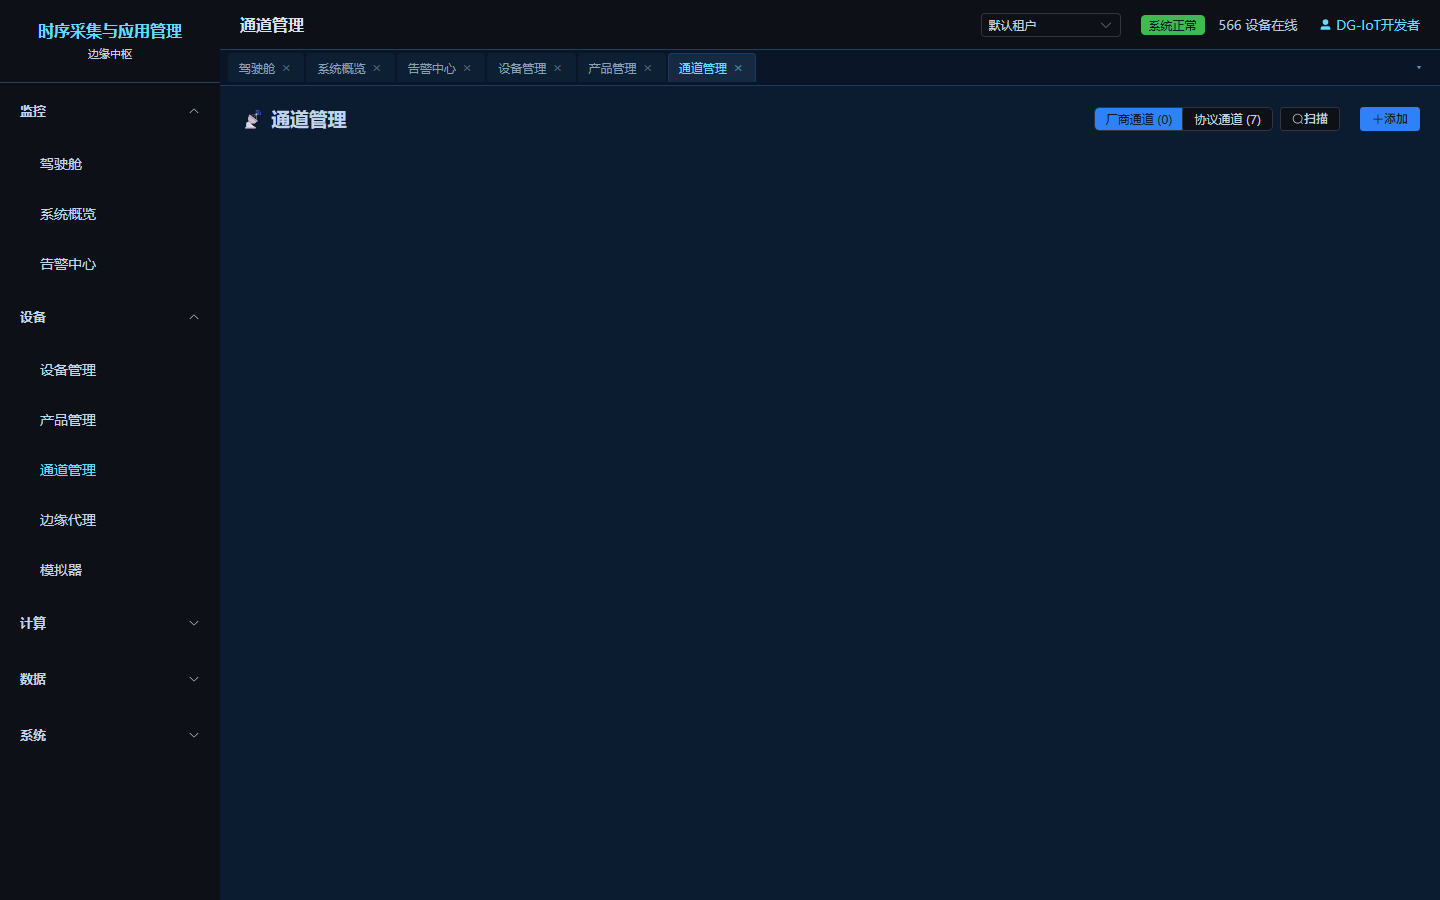
\includegraphics[width=0.95\textwidth]{all-fde.png}\caption{FDE六步工作法 -- 物模型→本体→协议→规则→驾驶舱→AI Agent}\end{figure}

\begin{figure}[H]\centering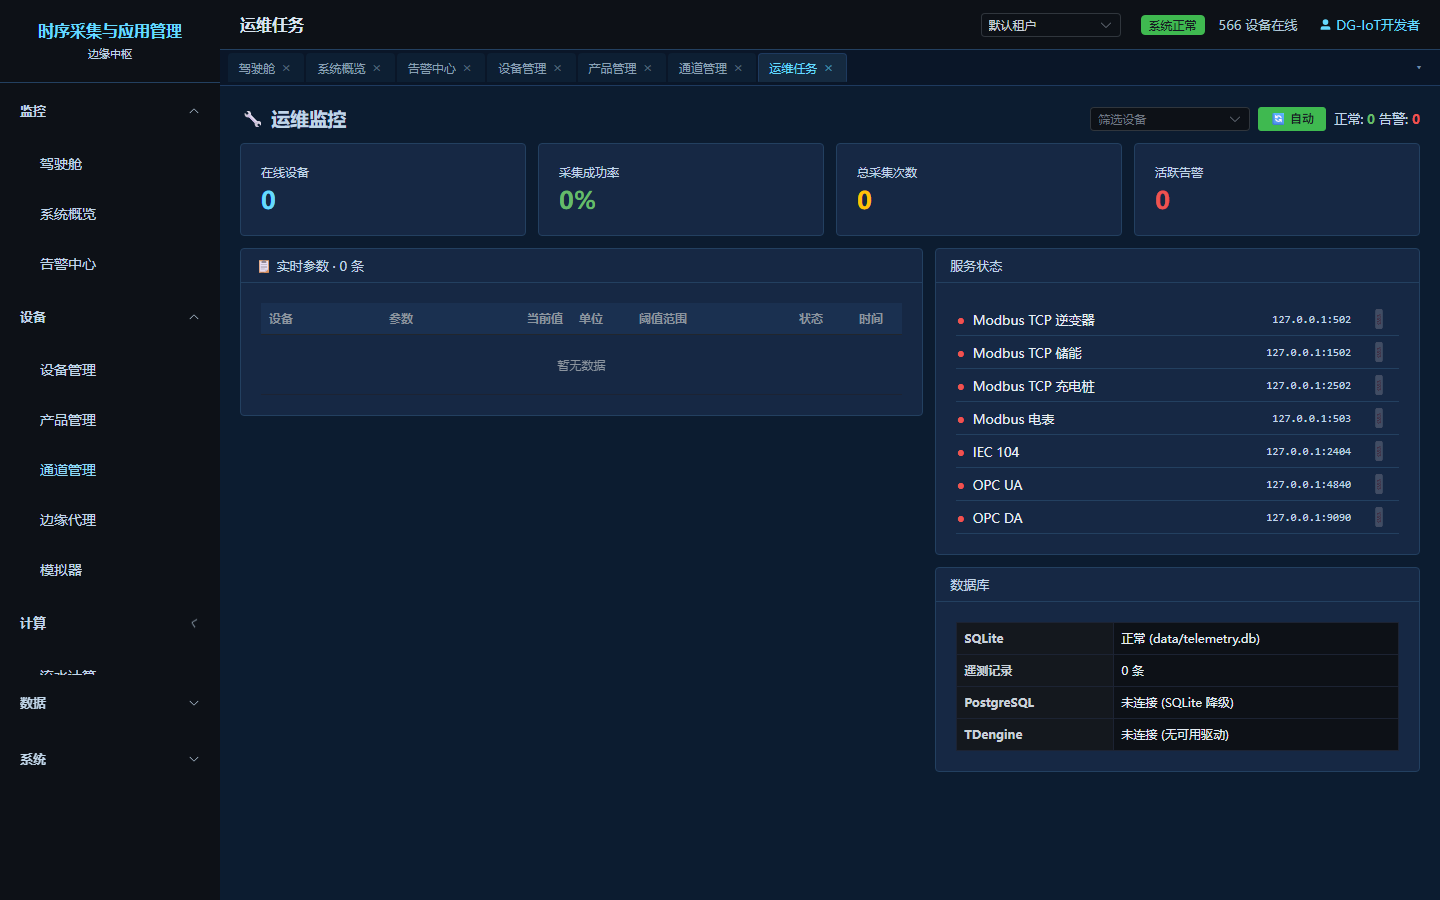
\includegraphics[width=0.95\textwidth]{all-maintenance.png}\caption{运维任务 -- 服务启停 · 实时参数 · 日志查看}\end{figure}

\section{数据组}

\begin{figure}[H]\centering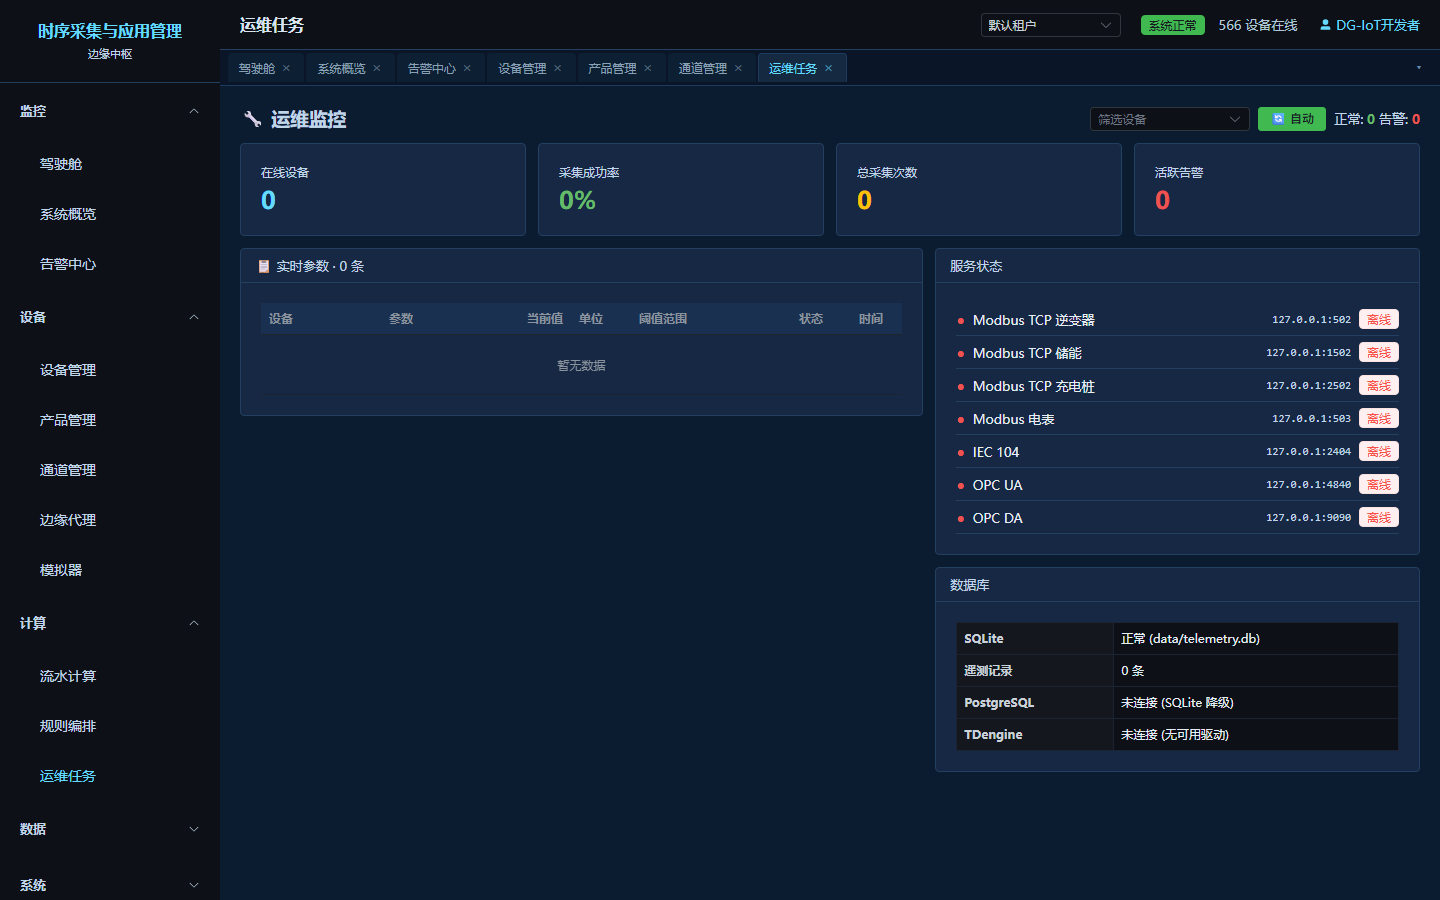
\includegraphics[width=0.95\textwidth]{all-reports.png}\caption{数据报表 -- 日月年聚合 · 曲线回放 · 排行导出}\end{figure}

\begin{figure}[H]\centering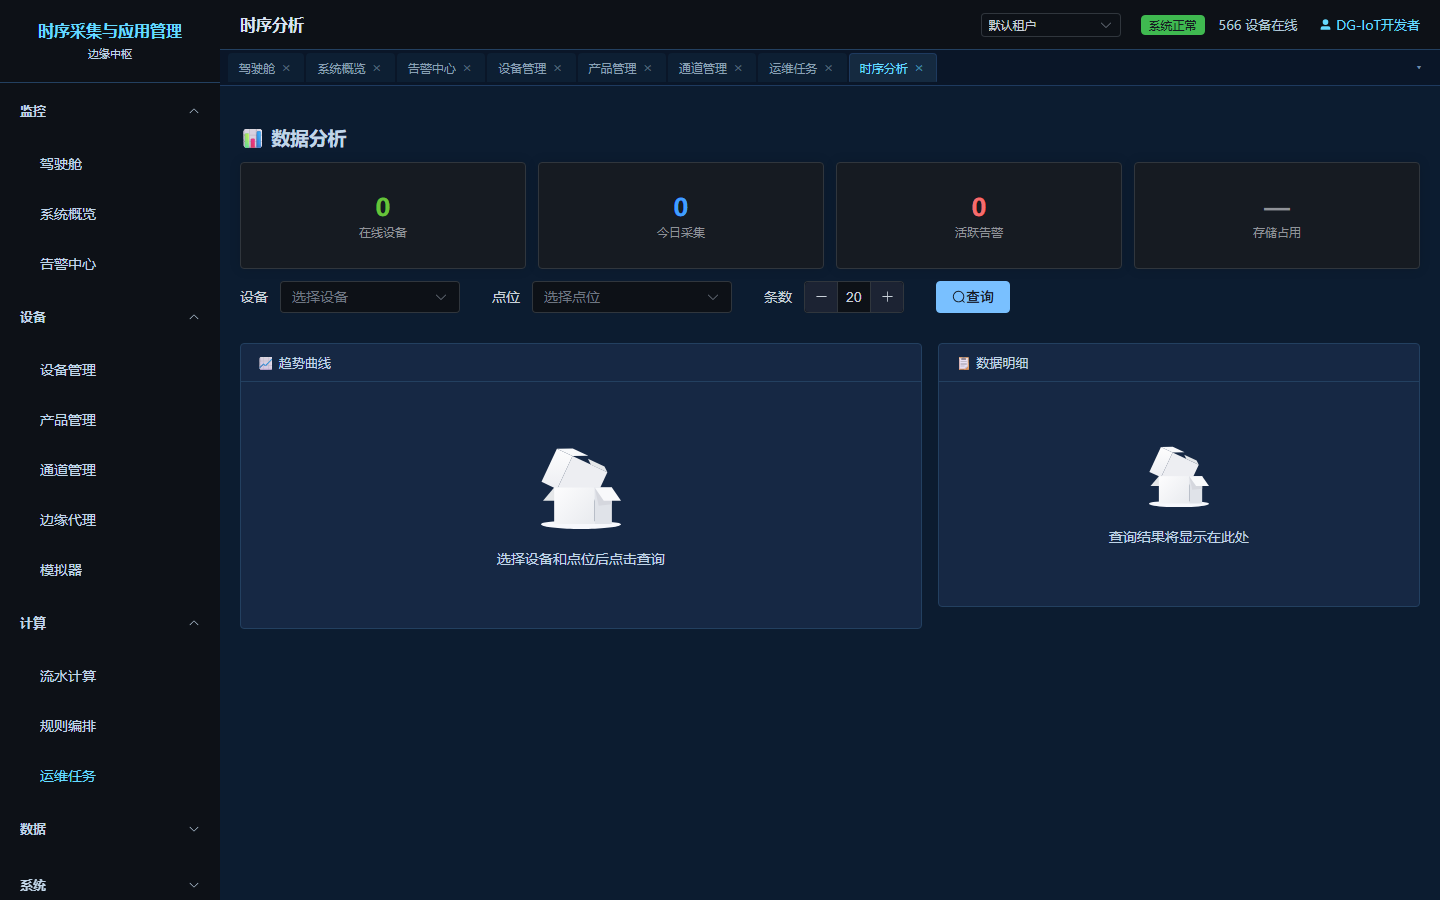
\includegraphics[width=0.95\textwidth]{all-telemetry.png}\caption{时序分析 -- 设备/点位选择 · 趋势曲线 · 数据明细}\end{figure}

\begin{figure}[H]\centering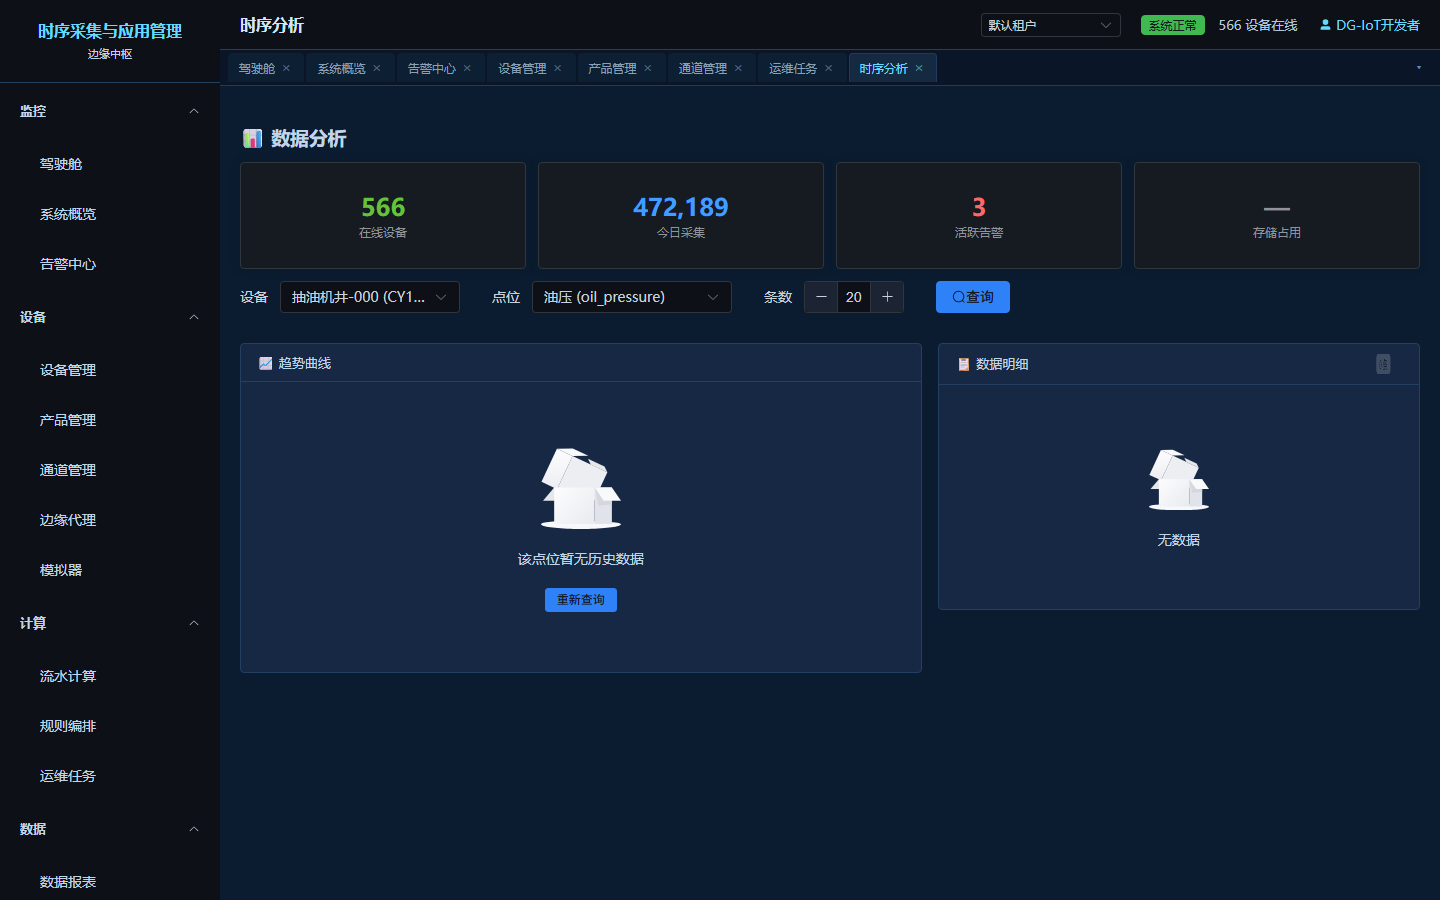
\includegraphics[width=0.95\textwidth]{all-topology.png}\caption{链路拓扑 -- 树导航+力导向图 · 油田→厂→作业区→间站}\end{figure}

\begin{figure}[H]\centering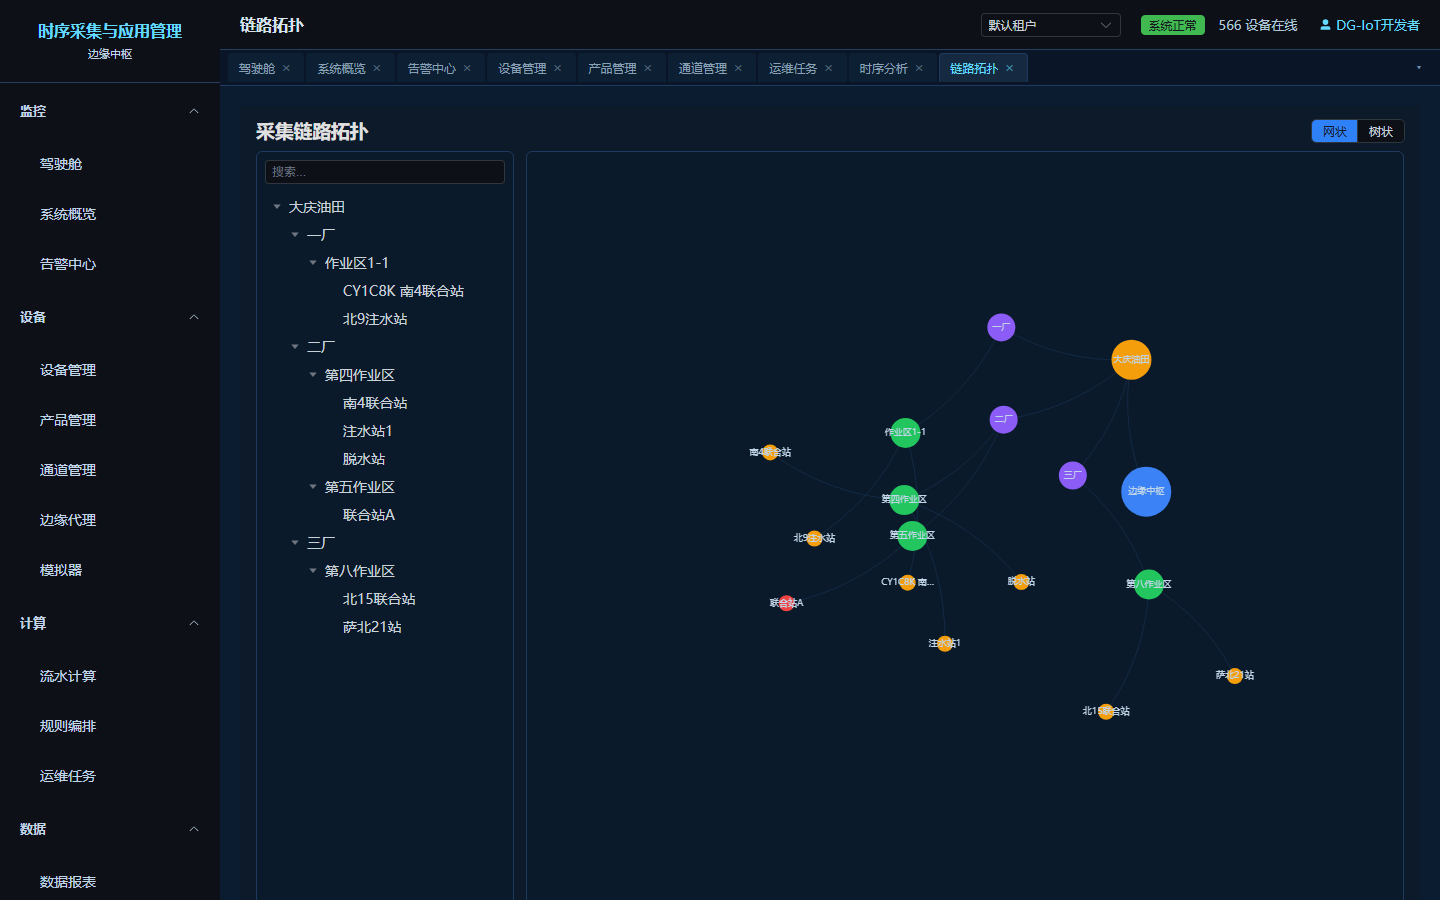
\includegraphics[width=0.95\textwidth]{all-scada.png}\caption{SCADA -- 2D组态编辑器 · 编辑/运行模式切换}\end{figure}

\begin{figure}[H]\centering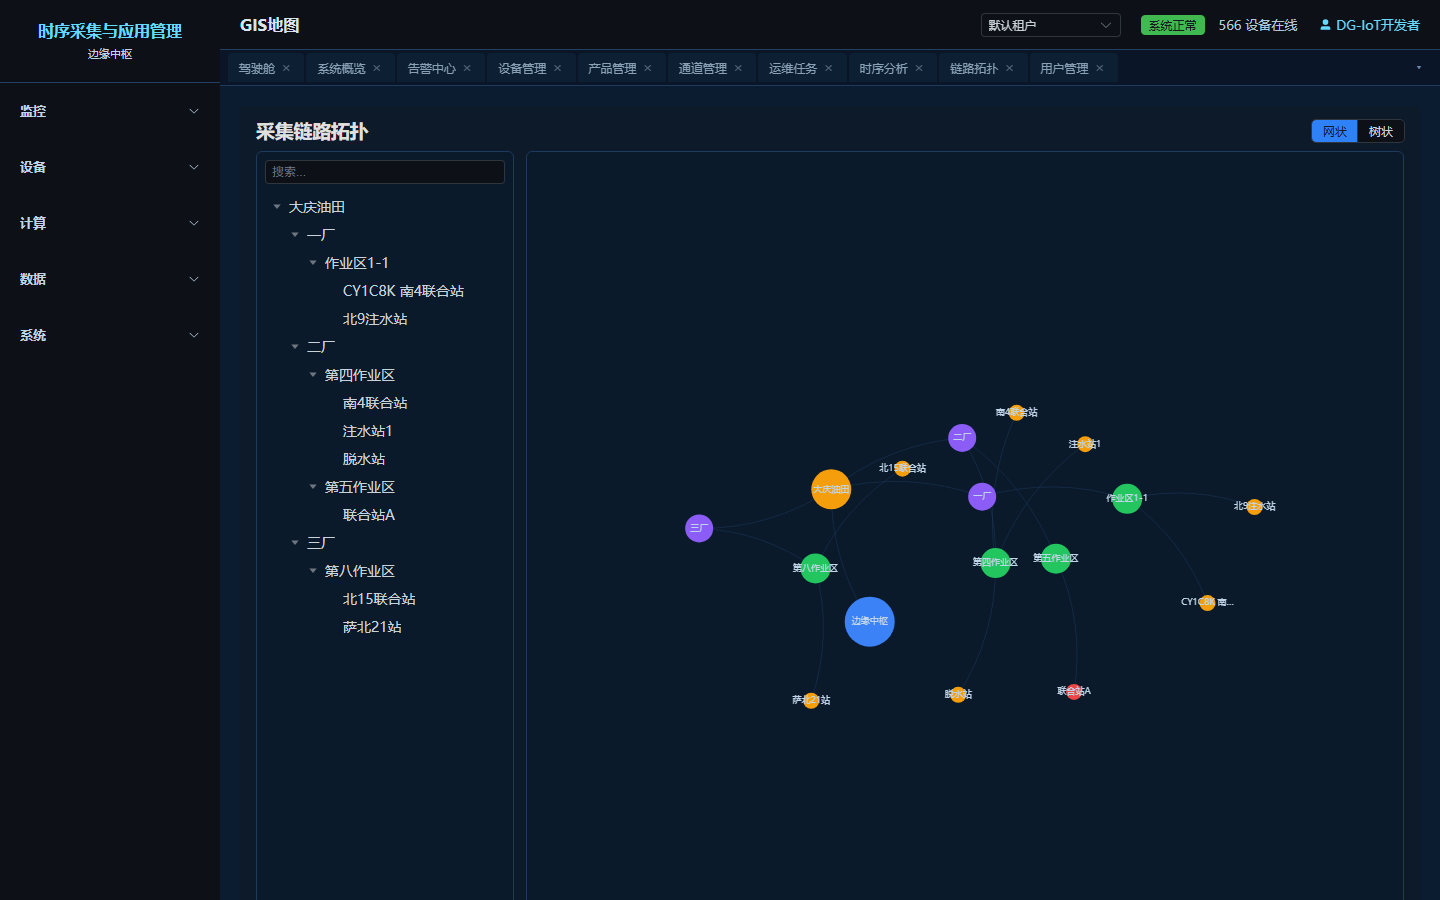
\includegraphics[width=0.95\textwidth]{all-gis.png}\caption{GIS地图下钻 -- 油田→16厂→作业区→间站 三级}\end{figure}

\section{系统组}

\begin{figure}[H]\centering
\includegraphics[width=0.95\textwidth]{all-users.png}\caption{用户管理 -- 3用户3角色 · 部门组织树 · 角色分配保存}\end{figure}

\section{页面清单}

\begin{table}[H]\centering
\begin{tabular}{p{2.5cm} p{3cm} p{7cm}}
\toprule
\textbf{组} & \textbf{页面} & \textbf{核心功能} \\
\midrule
监控 & 驾驶舱 & KPI·拓扑·告警滚动·秒级刷新 \\
 & 系统概览 & 服务健康·资源监控 \\
 & 告警中心 & 四级告警·确认清除·升级链 \\
设备 & 设备管理 & 566设备·六页签详情·五态生命周期 \\
 & 产品管理 & 12种产品·物模型属性 \\
 & 通道管理 & 7通道·在线离线状态 \\
 & 边缘代理 & 协议适配器·吞吐图·IO扫描 \\
 & 模拟器 & Modbus/OPC/IEC/A11启停 \\
计算 & 流水计算 & 15算法·定制注册·A/B对比 \\
 & FDE六步法 & 物模型→本体→协议→规则→AI \\
 & 运维任务 & 服务启停·日志查看 \\
数据 & 数据报表 & 日月年聚合·排行导出 \\
 & 时序分析 & 趋势曲线·数据明细 \\
 & 链路拓扑 & 树导航·力导向图 \\
 & SCADA & 2D组态编辑器 \\
 & GIS地图 & 油田→厂→区→站下钻 \\
系统 & 用户管理 & 3用户·角色分配·部门树 \\
\bottomrule
\end{tabular}
\end{table}

\end{document}
